\chapter{Architecture}

The Flutter framework is organized into a series of layers, with each layer building upon the previous layer\\\\
\begin{figure}[h]
  \begin{center}
  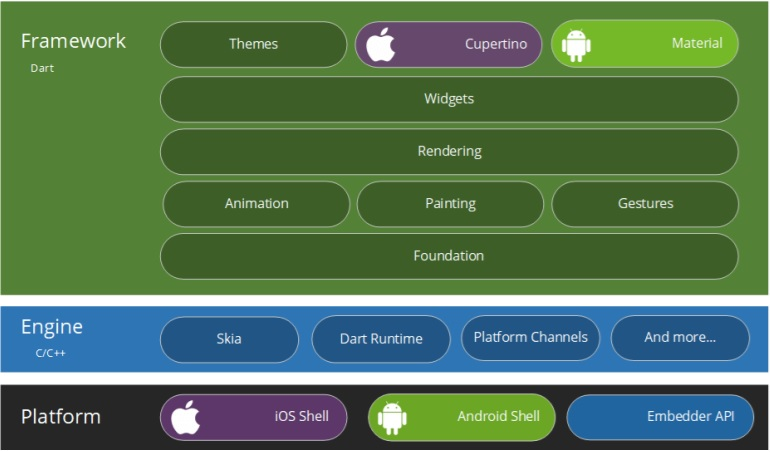
\includegraphics[height=80mm]{Images & Logos/CH_02_architecture.jpg}
  \end{center}
  \caption{Architecture of Flutter Framework}
\end{figure}  
  




\section{Dart Framework}

Flutter applications are written in the Dart language and utilize a considerable lot of the language's more
progressed highlights. On Android, and on Windows, macOS and Linux by means of the semi-official Flutter
Work area Embedding project, Flutter runs in the Dart virtual machine which includes an in the nick of time
execution engine. Because of App Store limitations on unique code execution, Flutter applications use ahead-of-time (AOT) compilation on iOS.\\
An outstanding element of the Dart stage is its help for "hot reload" where adjustments to
source documents can be infused into a running application. Flutter expands this with help for stateful hot
reload, where as a rule changes to source code can be reflected promptly in the running application
without requiring a restart or any deficiency of state.

\section{Flutter's Engine}
Flutter's Engine, composed essentially on C++, gives low-level rendering support utilizing Google's
Skia Graphics library. Furthermore, it interfaces with platform explicit SDKs, for example, those given
by Android and iOS.\\
The Flutter Engine is a compact runtime for facilitating Flutter applications. It executes Flutter's
core libraries, including activity and designs, file and network I/O, accessibility support, plugin architecture, and a Dart runtime and compile toolchain. Most engineers will associate with Flutter by means of
the Flutter Framework, which gives a cutting edge, responsive system, and a rich arrangement of stage,
design and establishment gadgets.

\section{Platform}
At the platform level, Flutter gives a Shell, that has the Dart Virtual Machine. The Shell, is platform
explicit, giving admittance to the local APIs and facilitating the building up the stage applicable
material. There is additionally an embedder API, to utilize Flutter like a library, rather than facilitating
running an application. The Shells, additionally assist with giving correspondence to the applicable IMEs and the frameworks
application lifecycle occasions.